\section{Vegetation}

Vegetation is core to rural landscapes. The species present along with their associated densities create a relationship between ecosystems and areas on earth on which resources are adequate. To ensure realism in virtual environments, much emphasize must be put on efficiently modelling these underlying ecosystems.\\

This section will review different methods to generate suitable vegetation for virtual worlds. These methods can be split into three main categories: \textit{Explicit Instancing, Probabilistic Instancing} and \textit{Plant Growth Modelling}.\\
\textit{Explicit Placement} require explicit user-input to directly or indirectly pinpoint exact locations for individual plant instances.\\
\textit{Probabilistic Placement} methods use statistical models to generate suitable vegetation.\\ 
\textit{Simulators} attempt to algorithmically reproduce plants battling for available resources.\\

We will measure the success of these techniques based on the level of automation they provide, the realism they achieve, their computational cost and their adaptability. Adaptability, here, represents the ease at which a given technique is able to model a number of different vegetative scenarios. \\

\subsection{Explicit Placement} \label{Explicit Placement}
Explicit placement methods require input from the user to determine the location and properties of individual plants. \\

Arnaud et al. \cite{Emilien} permit users to insert individual plants manually by simply clicking a given location on the terrain. To overcome the tedious task of manually placing individual plants on large terrains, the system is able to analyse existing distributions for reproduction. For example, to generate a large forest, the user is only required to generate a small subsection which can then be used to reproduce it on any scale (figure \ref{Explicit placement as input examplars}) \\

\begin{figure}[h]
  \centering
	\label{Explicit placement as input examplars}
	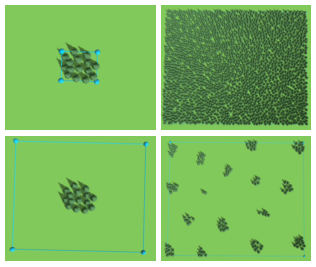
\includegraphics[natwidth=316,natheight=267]{worldbrush_forrest_reproduction.png}
	\caption{Using explicit placement as input examplars for reproduction \cite{Emilien}}
\end{figure}

Similarly, Deussen et al. \cite{Deussen1998} allow users to use grayscale raster images as input to specify terrain vegetation. The location of individual plants is determined by pixel location whereas plant properties are correlated to pixel intensity.\\

In their work focused on improving the realism of roadside landscapes, Andujar et al. ~\cite{Andujar2014} use orthophotos as input to determine the location and properties of individual plants. Unlike ordinary aerial photographs, aerial orthophotos use normalisation techniques to take into account terrain relief and camera tilt. The result is an image with uniform scale throughout which, similarly to a map, can be used to accurately measure distances between points. These orthophotos are used to measure the distances between plants. To later reproduce the roadside landscape, they use a dart throwing algorithm to place individual plants whilst respecting the appropriate distances. \\

\begin{figure}[!htb]
  \centering
	\label{Reconstructed roadside vegetation using orthophotos}
	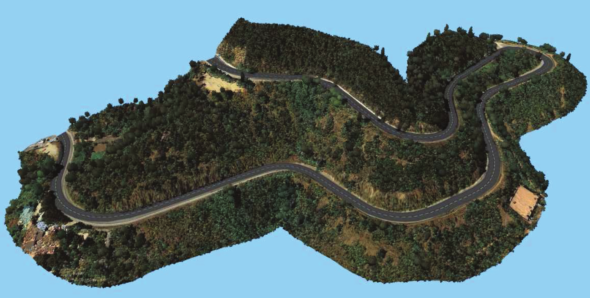
\includegraphics[width=\textwidth]{reconstructed_roadside_vegetation.png}
	\caption{Reconstructed roadside vegetation using orthophotos ~\cite{Andujar2014}}
\end{figure}

\subsubsection{CONCLUSIONS}

Explicit placement methods provide significant user control over the resulting virtual world. However, as there is \textit{little to no automation} of this process, it can be very tedious and time consuming for the user. This is especially true when the virtual world being created are very large (e.g. open world video games). An advantage of this limited automation, however, is that modifications are most often very small and are therefore performed in real-time. \\
The \textit{adaptability} of these methods are very poor. Running a different scenario would most often involve starting explicitly placing individual plants from scratch.\\
Creating vegetation for large virtual worlds using these methods is extremely strenuous and, as a consequence, realism is often compromised.

\subsection{Probabilistic Placement} \label{Probabilistic Placement}

Probabilistic placement methods use statistical models in an attempt to produce adequate vegetation. These methods can be further split into two sub-categories which are discussed in further detail below: \textit{Radial Distribution Analysis} and \textit{Predefined Ecosystems}.
\textit{Radial Distribution Analysis} approaches analyse the underlying distribution of the vegetation for later reproduction. \textit{Predefined Ecosystems} calculate, based on the varying resources of the terrain and a set of predefined ecosystems, the best suited. \\

\subsubsection{RADIAL DISTRIBUTION ANALYSIS}
Work by Emilien et al. \cite{Emilien}, Boudon et al. \cite{Boudon2007} and Lane et al. \cite{Lane2002} use radial distribution analysis to convert to metric form the underlying plant distributions of input examplars. The data generated by the analysis stage can later be used to synthesise, at any scale, new point distributions which respect the characteristics of the input exemplar. \\
For example, by analysing the positions of individual plants in a small subset of a forest and using it as the input exemplar, it is possible to reproduce it at a much larger scale in order to model its full size counterpart.\\

\paragraph{Analysis}
Generating the analytical data involves measuring the distances between individual points of different categories from the input examplar. For plant distribution analysis, the points represent individual plants and the categories represent the different species.\\

Before performing the analysis, the following parameters are configured:
\begin{itemize}
\item \textbf{R\textsubscript{min}}: The minimum distance from which point distances need to be analysed.\\
\item \textbf{R\textsubscript{max}}: The maximum distance after which point distances don't need to be analysed.\\
\item \textbf{Bin size}: When analysing the distances of given points, it is necessary to aggregate the points which reside at similar distances into bins. The bin size is the range represented by a single bin.\\
\end{itemize}

A core part of radial distribution analysis is generating pair correlation histograms for each category pair combination. A pair correlation histogram \textit{H\textsubscript{AB}} represents the variation in the distance between points of of category \textit{C\textsubscript{A}} and \textit{C\textsubscript{B}} ranging from \textit{R\textsubscript{min}} to \textit{R\textsubscript{max}} in \textit{bin size} increments (figure \ref{Pair Correlation Histograms}) \\

\begin{figure}[h]
  \centering
	\label{Pair Correlation Histograms}
	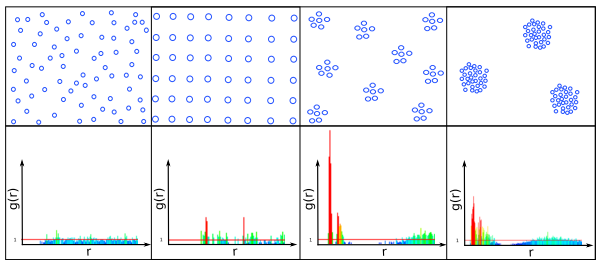
\includegraphics[width=\textwidth]{pair_correlation_histograms.png}
	\caption{Point distributions with associated pair correlation histogram \cite{Emilien2014}}
\end{figure}

To generate the pair correlation histogram \textit{H\textsubscript{AB}}, the algorithm iterates through each reference point of category \textit{C\textsubscript{A}} and, for each destination point of category \textit{C\textsubscript{B}} at a distance between \textit{R\textsubscript{min}} and \textit{R\textsubscript{max}}, increments the relevant bin in the histogram. In figure \ref{Radial distribution analysis}, for example, are being measured the points that lie within the annular shell of radius \textit{r} with bin size \textit{d\textsubscript{r}} (area \textit{d\textsubscript{A}}). 

\begin{figure}[h]
  \centering
	\label{Radial distribution analysis}
	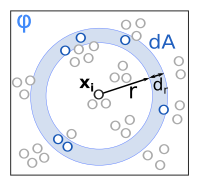
\includegraphics[natwidth=199,natheight=140]{radial_distribution_analysis.png}
	\caption{Radial distribution analysis}
\end{figure}

Because of their larger circumference, the coverage area of annular shells get larger as the distance bin being measured increases. In other words, \textit{A\textsubscript{r}} \textless \textit{A\textsubscript{r+1}} where \textit{A\textsubscript{r}} is the area covered by the annular shell starting at distance \textit{r}. A direct consequence of this is that annular shells at further distances will naturally be prone to containing more points. To counter for this, normalisation is performed based on annular shell area. \\

The radial distribution analysis function \textit{h\textsubscript{rdf}} is as follows:\\
\begin{center}	
$h_{rdf}(k) = \sum_{x_{i} \in X} \sum_{y_{j} \in Y \&  
kd_{r} \leq d(x_{i}, y_{j}) < (k+1)d_{r} } \frac{A}{d_{A}n_{x}n_{y}} $
\end{center}
Where:
\begin{itemize}
\item \textit{hrdf(k)} is the k-th value of the pair wise histogram.
\item \textit{X} are the points of category X (reference points).
\item \textit{Y} are the points of category Y (target points)    .
\item \textit{d\textsubscript{r}} is the annular shell width.
\item \textit{A} is the total analysed area.
\item \textit{n\textsubscript{x}} and \textit{n\textsubscript{y}} are the number of points of categories \textit{x} and \textit{y} respectively. Note that pairwise histograms also need to be calculated for points of the same category. In this situation, category \textit{x} and category \textit{y} would be the same.
\item \textit{d\textsubscript{A}} is the area of the annular shell being analysed.
\end{itemize}

Conceptually, this formula calculates the variance from the average density of the target category at incremental distances from points of the reference category.\\

\paragraph{Reproduction}

In order to reproduce the distribution of the input exemplar, points are added iteratively whilst matching as closely as possible the corresponding pair correlation histogram data calculated during the analysis stage. Metropolis-Hastings sampling ~\cite{Hurtut2009} is the most common way to do this. It involves performing a fixed number of point birth-and-death perturbations. A change from the initial arrangement \textit{X} to the new arrangement \textit{X'} is accepted with probability \textit{R}, where:

\begin{center}
$ R = \frac{f(X')}{f(X}$
\end{center}
\textit{f(X)} is the probability density function (PDF) of a given arrangement and is expressed as:\\

\begin{center}
$ f(X) = \prod_{C_{Y_{K}} \leq C_{X}} 
		 \prod_{x_{i} \in X}
		 \prod_{y_{i} \in Y_{k}} 
		 h_{X,Y_{k}}(d(x_{i},y_{j}))$
\end{center} 

Where:
\begin{itemize}
\item \textit{C\textsubscript{y}} and \textit{C\textsubscript{x}} represent categories \textit{Y} and \textit{X}, respectively.
\item \textit{X} are all points of category \textit{X}.
\item \textit{Y} are all points of category \textit{Y}/
\item h\textsubscript{X,Y\textsubscript{k}}(d(x\textsubscript{i}, y\textsubscript{j})) is the value retrieved from the pairwise histogram of categories \textit{X} and \textit{Y} given the distance between points \textit{x\textsubscript{i}} and \textit{y\textsubscript{i}}.
\end{itemize}
Intuitively, the PDF defines, given a set of points, the aggregate strength of the current distribution.\\

Because the PDF formula is a product, calculating it for a new layout \textit{X'} with appended/removed point \textit{P} only involves calculating the PDF for the single reference point \textit{P}. As a consequence, reproduction can be performed very efficiently. In their work, Emilien and Cani ~\cite{Emilien} are able to perform analysis and reproduction in near real-time.\\

When using this technique to reproduce a plausible plant distribution, Boudon et al. \cite{Boudon2007} take it one step further by enabling plant crowns to deform based on predefined elasticity parameters. Because the crowns are not constrained to being circular, they can deform to permit facilitate the survival of plants at a lower height.

\subsubsection{PREDEFINED ECOSYSTEMS}
In their work, Hammes el al. \cite{Hammes2001} predefine ecosystems along with their preferred environment. These environments are defined in terms of:

\begin{itemize}
\item Elevation: All plant species have an upper limit after which temperature or oxygen levels are ill-suited.
\item Relative elevation: The local changes in height. Local minimums tend to be valleys and therefore wetter with less illumination. Local maximums, on the other hand, tend to me ridges which are dryer and much more exposed.
\item Slope: Gradient has a direct impact on the quality of the soil and therefore the plants which can grow. When slopes get steeper, plants tend to get much smaller as they struggle to get required nutrients from the soil.
\item Slope direction: This has a direct effect on sunlight exposure. Southern facing slopes in the northern hemisphere will have a greater exposure to the sun and vice-versa for the southern hemisphere.  
\end{itemize}

All these ecosystems are stored in a database and, when vegetation is to be placed on the terrain, the most suitable ecosystems are chosen based on the terrain properties mentioned above. See figure \ref{Vegetation generated using predefined ecosystems} for an example landscape generated using this technique.

\begin{figure}[h]
  \centering
	\label{Vegetation generated using predefined ecosystems}
	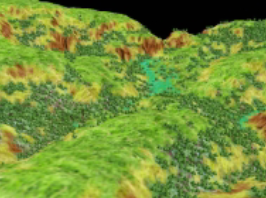
\includegraphics{predefined_ecosystems.png}
	\caption{Vegetation generated using predefined ecosystems \cite{Hammes2001}}
\end{figure}

\subsubsection{CONCLUSIONS}

\textit{Probabilistic Placement} permit users to specify only small portions of input data to populate large areas. For the \textit{Radial Distribution Analysis} approach, this input data would be in the form of an input distribution. For the \textit{Predefined Ecosystems} approach, it would be a predefined ecosystem along with its preferred environment. Although this automation does ease the task for artists, specifying accurate input data is still crucial to produce realistic vegetation. Consequently, although the realism achieved by these methods is generally good, their adaptability is still limited. \\
Thanks to the use of efficient algorithms, the computational complexity of these methods are often low and real-time updating is achievable. 

\subsection{Simulators} \label{Simulators}

Another approach used to determine vegetation in a given environment is to simulate plants battling for available resources. This approach can be further classified into two subcategories: \textit{Plant Growth Modelling} and \textit{Ecosystem Simulators}.\\
\textit{Plant Growth Modelling} techniques go into extensive detail to model the effect of resources on plant growth. The realism is such that it can often be used to model plant growth on earth. \\
\textit{Ecosystem Simulators} try to simulate plants competing for available resources when growing. Unlike plant growth modelling which targets botanical realism, these techniques target visual realism. As a consequence, they are more lenient in terms of realism.

\subsubsection{PLANT GROWTH MODELLING}

These types of simulators attempt to algorithmically reproduce the laws of nature with such precision that they can be used in agronomical sciences and forestry to estimate and maximize crop yield. To achieve this, such simulators go into great detail to model the available resources. For example,  work by Soler et al. ~\cite{Soler2001,Soler2003} splits single plants into geometrical organs with unique light transmittance and reflectance properties. By doing so, light propagation within the plant can be simulated in order to determine the aggregated photosynthetic potential. This work, along with that of Yan et al. ~\cite{Yan2004}, base their simulators on two vital and widely accepted laws of nature:

\begin{itemize}
\item \textit{Law of the sum of temperatures}: Plants grow in cycles which vary from days to years depending on the specie. The law of the sum of temperatures states that the frequency of these cycles is proportional to the sum of the daily average of the temperatures.
\item \textit{Law of the water use efficiency}: The amount of fresh matter fabricated by a plant is proportional to the water evaporation of the plant. This factor is called the water use efficiency. 
\end{itemize}

Water evaporates during photosynthesis as the plant exchanges water for carbon dioxide. Based on this and the law of water use efficiency outlined above, the amount of fresh matter produced (i.e growth) for a given plant is directly correlated to the amount of photosynthesis performed. Using this, Soler et al. ~\cite{Soler2001} apply the following formula to calculate the amount of fresh matter, \textit{Q\textsubscript{m}(t)}, created by a given plant at time \textit{t}:\\

\begin{center}	
\textit{$Q_{m}(t)$} = $\sum_{x=1}^{N(t)} \frac{E(x,t)}{R} $
\end{center}
Where:
\begin{itemize}
\item \textit{E(x,t)} is the potential for matter production of the \textit{x}-th leaf at the \textit{t}-th cycle. It is proportional to the incoming radiant energy up to a certain threshold, after which it remains constant. 
\item \textit{R} is the hydraulic resistance of the given leaf. This resistance is what limits water evaporation (photosynthesis) and therefore growth. It varies depending in the specie and surface area.
\end{itemize} 
Intuitively, this formula calculates the total available fresh matter, \textit{$Q_{m}$}, that can be produced for an individual plant \textit{P} at a given time \textit{t}, by calculating the photosynthesis potential of each individual leaf of \textit{P} given the current lighting.\\

Using this, the algorithm iterates through growth cycles with a frequency that is calculated based on the \textit{law of the sum of temperatures} mentioned above. Each growth cycle performs the following two steps:
\begin{enumerate}
\item The lighting and therefore photosynthesis potential of each individual leaf of the plant is calculated. This is then used to calculate, as above, the quantity of fresh matter produced.
\item The fresh matter is then distributed to different organs of the plant according to an associated organ strength.
\end{enumerate}

By going into such detail, these simulators produce very realistic simulations of the evolution of plants. For example, to maximize growth, plants are able to grow in direction of the light source (figure \ref{Plant growing towards light source}).\\

\begin{figure}[h]
  \centering
	  \label{Plant growing towards light source}
	    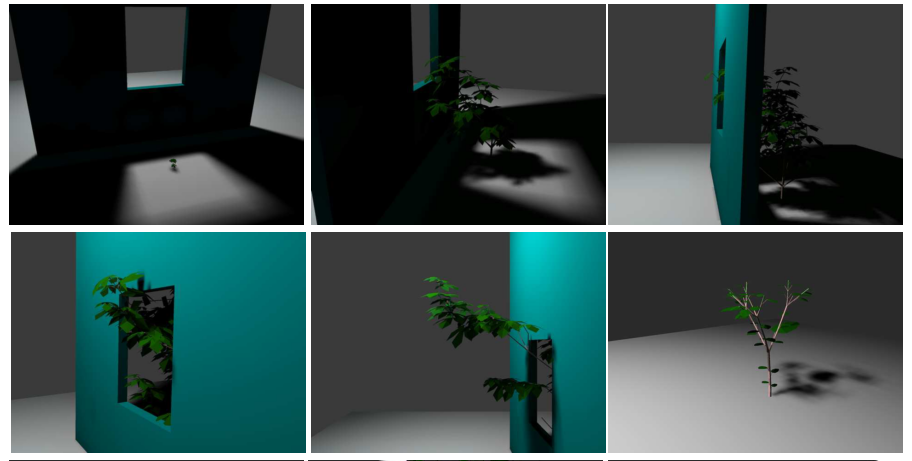
\includegraphics[width=\textwidth]{plant_growing_towards_light_source.png}
	\caption{Plant growing towards light source ~\cite{Soler2001} }
\end{figure}

\subsubsection{ECOSYSTEM SIMULATORS}

Ecosystem simulators use procedural methods to algorithmically reproduce the competition for resources that occurs in nature during plant growth. In nature, this competition is an extremely complex process and so reproducing it exactly would be infeasible. Instead, a simplified model of this ecological process is implemented. During these simulations, available resources fluctuate and each plants strength is continuously recalculated based on its associated properties. This strength directly affects the plants growth and chance of survival. \\
Such plant properties include: age; vigor; shade tolerance; humidity requirement and temperature requirements. Amongst others, the resources modelled include: available illumination; available humidity; temperature and slope.

The aim of ecosystem simulators is to determine, given an initial state \textbf{\textit{S\textsubscript{t}}} of the system at time \textbf{\textit{t}} and a simulation time \textbf{\textit{n}}, the state \textbf{\textit{S\textsubscript{t+n}}}. \\
The state of the system represents individual plant instances with associated location and properties. \\

Lindenmayer systems, commonly referred to as L-systems, use a formal grammar along with a set of production rules to iteratively create larger strings from a starting string called the axiom. Such systems are commonly used to model plants and plant growth ~\cite{Prusinkiewicz1990,Deussen2002,Boudon2012,Prusinkiewicz1993}. \\
An extension to basic L-systems, referred to as open L-systems, adds a communication grammar which permits the set of production rules to behave differently depending on predefined conditions ~\cite{Prusinkiewicz1996}. In their work modelling the growth of struce trees, Berezovskava et al. \cite{Berezovskava1997} use different production rules depending on local bud density. This is a simplified representation of buds competing for available light. \\

By introduction multiset L-Systems, Lane and Przemyslaw ~\cite{Lane2002} extend L-systems yet further to model an ecosystem simulator. The production rules for multiset L-systems work in two stages. The first, identical to basic L-Systems, produces a new string given an input string and production rule. The second, splits the resulting string into new sets using a predefined separation symbol. In their work, the different sets represent different plant instances, thus enabling new plants to spawn during the production steps. When building their L-System, Lane and and Przemyslaw ~\cite{Lane2002} focus on reproducing three important properties of nature, each distinctly testable to determine the plausibility of the results:
\begin{itemize}
\item \textit{Self-thinning}: When plants grow, their resource requirements increase and, as a direct consequence, inter-plant competition for resources increases. Eventually, the competition becomes too intense and resources too scarce leading to more vigorous plants starving smaller plants. At this point, self thinning begins and plant densities decrease.
\item \textit{Succession}: Given plant specie \textit{A} with a fast growth rate and specie \textit{B} with a slower growth rate but higher shade tolerance. At first, the faster growing specie \textit{A} will dominate and flourish but, with time, the slower growing but more shade tolerant specie \textit{B} will flourish and dominate.
\item \textit{Propagation}: Plants often propagate in clusters surrounding the seeding plant.
\end{itemize}

The L-System they implemented contains different production rules to represent the different properties of nature mentioned above. A single simulation and the corresponding output can be seen in figure ~\ref{Plant placement using an ecosystem simulator modelled by L-System}.

\begin{figure}[h]
  \centering
    \label{Plant placement using an ecosystem simulator modelled by L-System}
    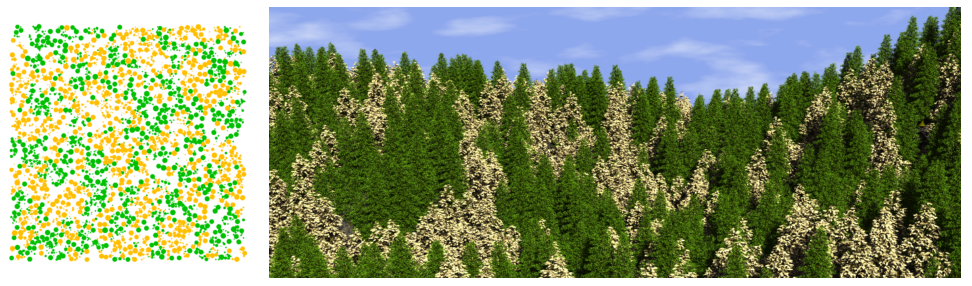
\includegraphics[width=\textwidth]{L-System-Result.png}
    \caption[Plant placement using an ecosystem simulator modelled by L-Systems]{ Plant placement using an ecosystem simulator modelled by L-Systems ~\cite{Lane2002}. \textit{Left:} Result of the simulation where orange circles indicate the positions of poplar trees and green circles the positions of spruce trees. \textit{Right:} Reproduced virtual world where the location of individual plants is deduced from the output of the simulator.}
\end{figure}

Work by Deussen et al. ~\cite{Deussen1998} also uses L-Systems as the basis for an ecosystem simulator. As an extension to the work by Lane and Przemyslaw ~\cite{Lane2002}, they introduce the notion of soil humidity and an associated soil per specie humidity preference.

A direct consequence of the automation provided by these ecosystems is that fine control over the final vegetative content is lost. Deussen et al. ~\cite{Deussen1998} overcome this, however, by offering a hybrid approach where the ecosystem simulator is first used to populate the entire terrain and explicit instancing is used thereafter for the detailing .\\

Another weakness of procedural ecosystems based on L-Systems worth mentioning is that the communication parameter is binary; in the work by Lane et al. ~\cite{Lane2002} a plant will be dominated as soon as it’s radius intersects another larger plant, at which point it will die with a set probability. This probability of death will stay constant and will not increase as this domination increases. Similarly, in the humidity model of Deussen et al. ~\cite{Deussen1998}, a plant has a preference for wet or dry areas and there is no notion of a measurable humidity preference range. This could prove problematic to model species which are able to adapt to a multitude of environments with varying resource availability (e.g. grass). \\

\subsubsection{CONCLUSIONS}
Probably the main advantage of simulators over other approaches is the level of \textit{automation}. Running simulations is done with easy and requires very little input from the user. \\
Although the adaptability of these methods is also impressive, it is limited by the necessity to configure the properties for individual species. This is especially true for \textit{Plant Growth Modelling} approaches where topological data must be configured. Obtaining topological data often involves real-world analysis of the plants growth cycles. \\
Computational cost is often high when using simulators. The extent of which is dependant on the level of detail and the number of plants being simulated simultaneously. For example, in the highly detailed simulations of Soler et al. ~\cite{Soler2001}, simulating 45 cycles for a single plant takes approximately 15 minutes.\\

\subsection{Conclusions} \label{Conclusions}

Which technique (Explicit, Probabilistic or Simulators) to use entirely depends on the requirements of the system. For example, if realism is the key priority then ecosystem simulators able to provide botanical realism would be the most suitable approach. Choosing the technique is therefore all about minimizing the associated compromises. In table \ref{Probabilistic Placement} we summarize the pros and cons of the individual techniques based on the following criteria: 
\begin{itemize}
\item \textit{Automation}: The level of automation the technique provides. That is, how little user input is needed.
\item \textit{Realism}: The level of realism with which the technique models real-world ecosystems.
\item \textit{Computational efficiency}: The techniques efficiency in terms of computational resource requirements.
\item \textit{Adaptability}: How well the technique can adapt to model different scenarios.
\end{itemize}
\begin{table}[h]
  \centering
	  \label{Pros and cons of individual techniques}
	    \begin{tabular}{|p{4cm}|p{3cm}|p{3cm}|p{3cm}|p{3cm}|}
  	    \hline	
  	      & \textbf{Automation} & \textbf{Realism} & \textbf{Computational Efficiency} & \textbf{Adaptability} \\
		\hline	
		\textbf{Explicit Placement} & 
		 %Automation  %Realism  %Comp. Effic. %Adaptability
		 Poor  & Poor  & Excellent & Poor      \\
  	    \hline	
  	    \multicolumn{5}{|c|}{\textbf{Probabilistic Placement}} \\
  	    \hline				
  	    \textbf{Radial Distribution Analysis} & 
		 %Automation  %Realism  %Comp. Effic. %Adaptability
		 Good & Very Good & Very Good & Fair   \\
  	    \hline
		\textbf{Predefined Ecosystems} & 
		 %Automation  %Realism  %Comp. Effic. %Adaptability
		 Good & Fair & Very Good & Poor      \\
  	    \hline
		\multicolumn{5}{|c|}{\textbf{Simulators}} \\
  	    \hline		
		\textbf{Plant Growth Modelling} & 
		 %Automation  %Realism  %Comp. Effic. % Adaptability
		 Excellent & Excellent & Poor & Fair  \\
  	    \hline
		\textbf{Ecosystem Simulators} & 
		 %Automation  %Realism  %Comp. Effic. %Adaptability
		 Excellent & Very Good & Fair & Good   \\
  	    \hline
  	    \end{tabular}
  \caption[Pros and cons of individual techniques]{Pros and cons of individual techniques}
\end{table}

Given a set of plant species, available resources and terrain, our system must be able to specify the locations of individual plants. The output must be: visually realistic; easily scalable in order to be able to re-run simulations with different input species; computationally efficient to ensure the effect of user actions appear in close to real-time. \\
Given these requirements, a hybrid approach is best suited which combines the adaptability and realism of ecosystem simulators with the computational efficiency of probabilistic placement. Computationally expensive ecosystem simulator runs will be performed beforehand in order to acquire the necessary distribution data. This data will then be stored in order for it to be queried at a later stage without having to redo expensive simulations. When placing vegetation in the virtual world, pre-calculated distribution data will be queried and probabilistic instancing used to fill user-defined areas with suited plant species and realistic distributions. \\